\subsection{Диаграмма последовательности программного средства}
\label{sec:modeling:sequence}

Диаграмма последовательности (Sequence Diagram) – диаграмма, на которой показаны взаимодействия объектов, упорядоченные по времени их проявления.

Основными элементами диаграммы последовательности являются обозначения объектов (прямоугольники), вертикальные линии, отображающие течение времени при деятельности объекта,и стрелки, показывающие выполнение действий объектами. На данной диаграмме объекты располагаются слева направо. Ее недостатком является то, что она занимает много места.

Диаграммы последовательности, описывающие сценарии Business Use Case в виде последовательности обмена сообщениями между объектами - действующими лицами и объектами-исполнителями. Такие диаграммы помогают явно определить в модели обязанности каждого исполнителя в виде набора операций класса.

На диаграмме последовательности изображаются только те объекты, которые непосредственно участвуют во взаимодействии. Ключевым моментом для диаграмм последовательности является динамика взаимодействия объектов во времени.

В UML диаграмма последовательности имеет как бы два измерения. Первое слева направо в виде вертикальных линий, каждая из которых изображает линию жизни отдельного объекта, участвующего во взаимодействии. Крайним слева на диаграмме изображается объект, который является инициатором взаимодействия. Правее изображается другой объект, который непосредственно взаимодействует с первым. Таким образом, все объекты на диаграмме последовательности образуют некоторый порядок, определяемый очередностью или степенью активности объектов при взаимодействии друг с другом.

\begin{figure}[ht]
\centering
    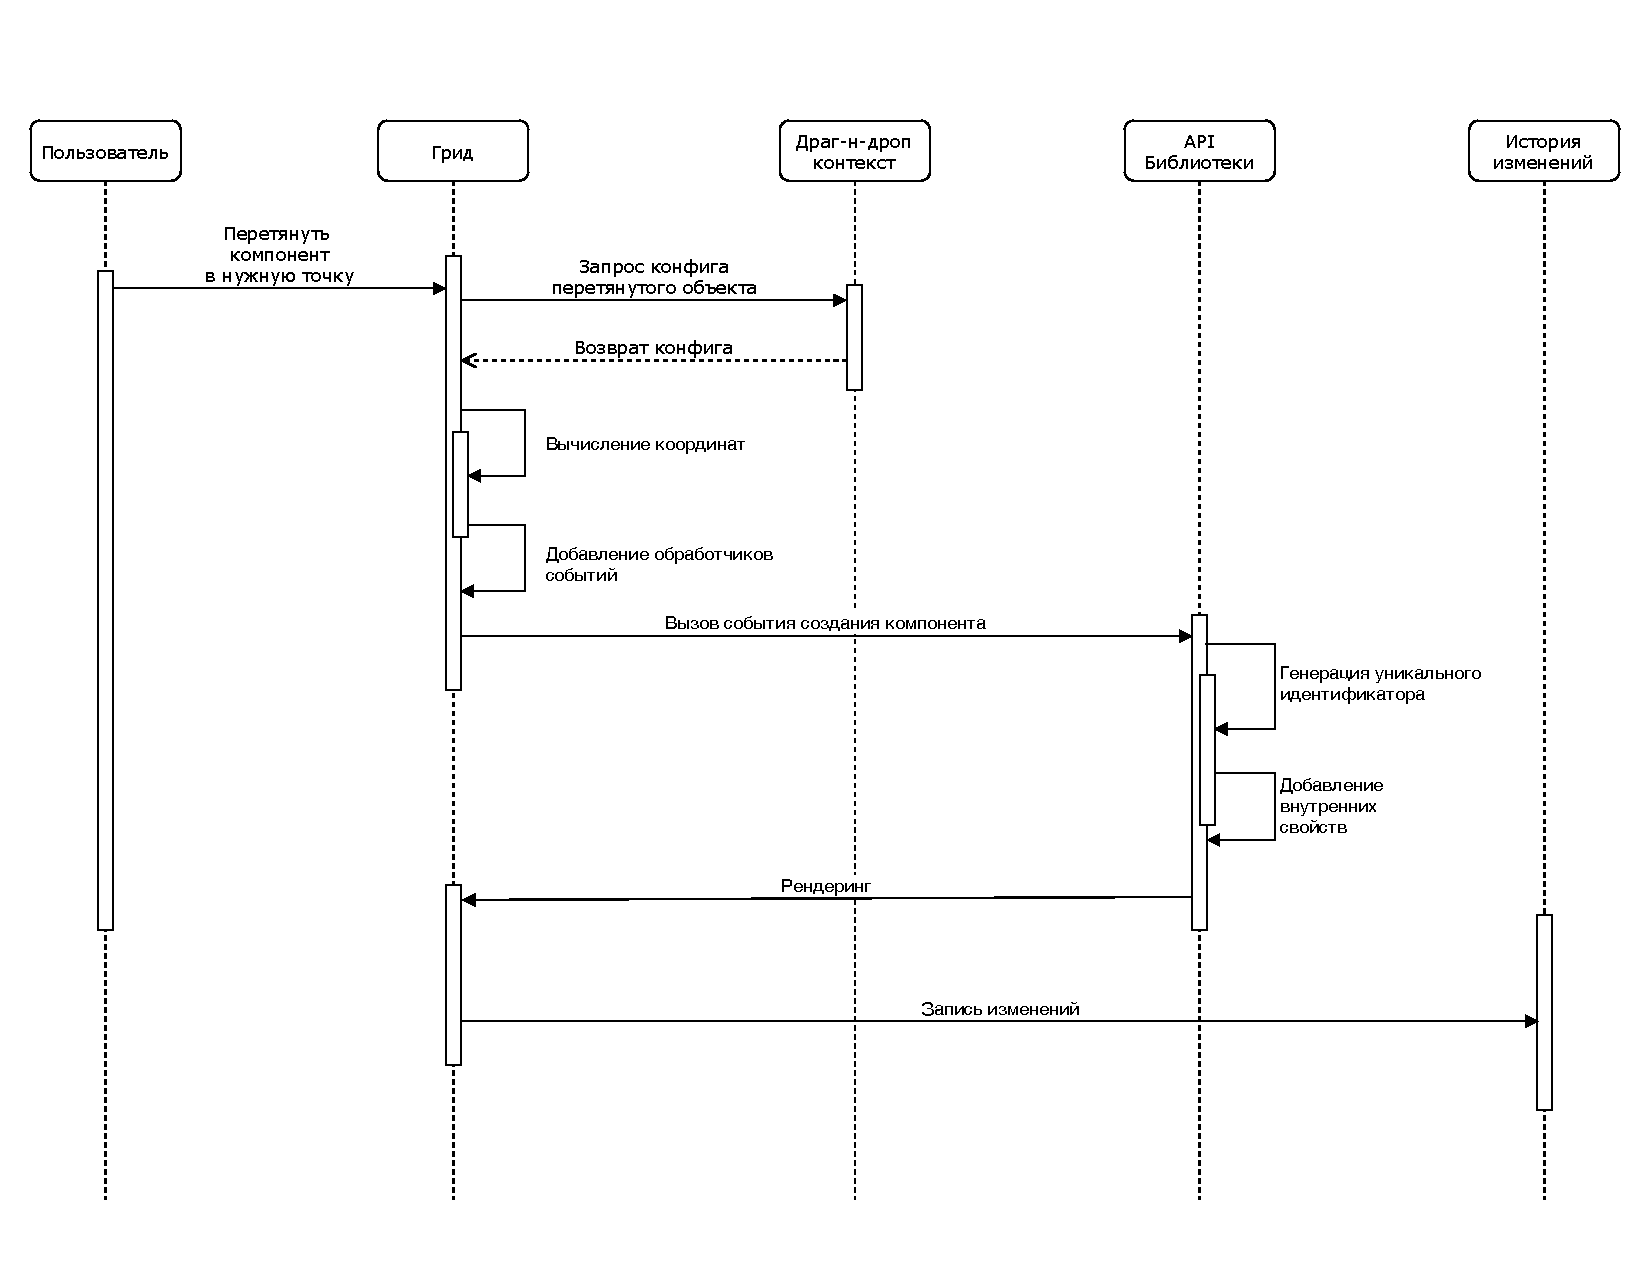
\includegraphics[scale=0.59]{Sequence.pdf}
    \caption{Диаграмма последовательности использования предопределенных конфигураций графических компонентов}
    \label{sec:design:sequence_diagram}
\end{figure}

На рисунке~\ref{sec:design:sequence_diagram} представлена диаграмма последовательности применения предопределенных конфигураций графических компонентов программного средства создания веб-приложений с помощью готовых графических компонентов. 
На ней отражен процесс, происходящий в программе каждый раз при перетягивании пользователем компонента на грид.\pagebreak

